\chapter{边缘智能裂缝检测算法设计与实现}
本章对边缘智能裂缝检测领域面临的问题和挑战、本文提出的检测算法和相应的实验及结果分析做出详细介绍。

%————————————————————————————————————————————裂缝检测问题分析—————————————————————————————————————————————————————————————————————————
\section{裂缝检测问题分析}
本文在第一章绪论的1.1节有关研究背景及意义的最后,提出了目前裂缝检测领域面临的两点难题和挑战:

第一,在算法层面,目前业界提出的深度学习模型较多关注于检测精度、鲁棒性的提升,导致模型尺寸越来越大,模型参数越来越多,而忽视了模型的轻量化和检测速度的提高,这对于路面检测实际应用
场景十分不利。
路面检测模型推理的时延和帧率,直接决定了公路检测车的行驶速度,直接影响路政部门进行路面检测的工作效率。
较高的检测速度和帧率,能够提高检测车的行驶速度,提升路面裂缝检测的工作效率。

第二,在系统层面,目前业界提出的裂缝检测系统多是基于云端高算力环境进行设计和部署,公路检测车需要将采集的图像数据上传至云端进行推理和识别,
既对算力和资源要求高,提高检测的成本,又增加了检测的通信时延,还存在中心服务器负载过高和部分重要场景隐私数据泄露的隐患。因此,
亟需将推理检测模型下发至检测车本地进行部署,以降低检测成本、提高检测速度、减轻中心服务器负载和保护重要数据隐私。

针对上述两方面的难点和挑战,本文充分考虑道路裂缝检测实际场景精度和速度的双重需求,设计并实现了一套边缘智能道路裂缝检测系统。
该系统设计并部署实现了基于U-Net卷积神经网络的裂缝检测算法,用于路面裂缝的分割和识别。

%————————————————————————————————————————————基于U-Net的边缘智能裂缝检测算法设计—————————————————————————————————————————————————————————————————————————
\section{基于U-Net的边缘智能裂缝检测算法设计}

\subsection{分割网}
计算机视觉领域的深度学习算法主要分为目标检测网、图像分类网和图像分割网。

检测网、分类网,是对图像“区域级”特征进行提取,并给出相应区域存在目标或者类别的概率,从而实现裂缝及其位置的检测。
该类算法关注的是图像的语义信息的提取,而无法兼顾具体像素级的位置信息的提取和还原,只能实现裂缝目标或类别的检测,而无法精准识别出裂缝的大小、形状和病害程度。

分割网,是对图像进行“像素级”的分类和语义分割,将采集的图像从像素水平上分割为裂缝和背景两类,从而实现更加精准的裂缝检测和识别。
相比检测网和分类网,分割网不但关注图像的语义类别信息,而且关注精确的位置信息,这十分有利于精确识别裂缝大小、形状及其病害程度,为后续路政部门决策提供更加精准的裂缝检测服务。

\subsection{U-Net整体结构}
U-Net卷积神经网络\citing{unet}是一种经典的图像分割网,最初由Olaf Ronneberger等人提出,并用于生物医学图像分割,取得不错的分割效果。

U-Net卷积网分为编码器Encoder和解码器Decoder两个部分,U-Net的网络结构示意图,见下图所示:

\begin{figure}[h]
	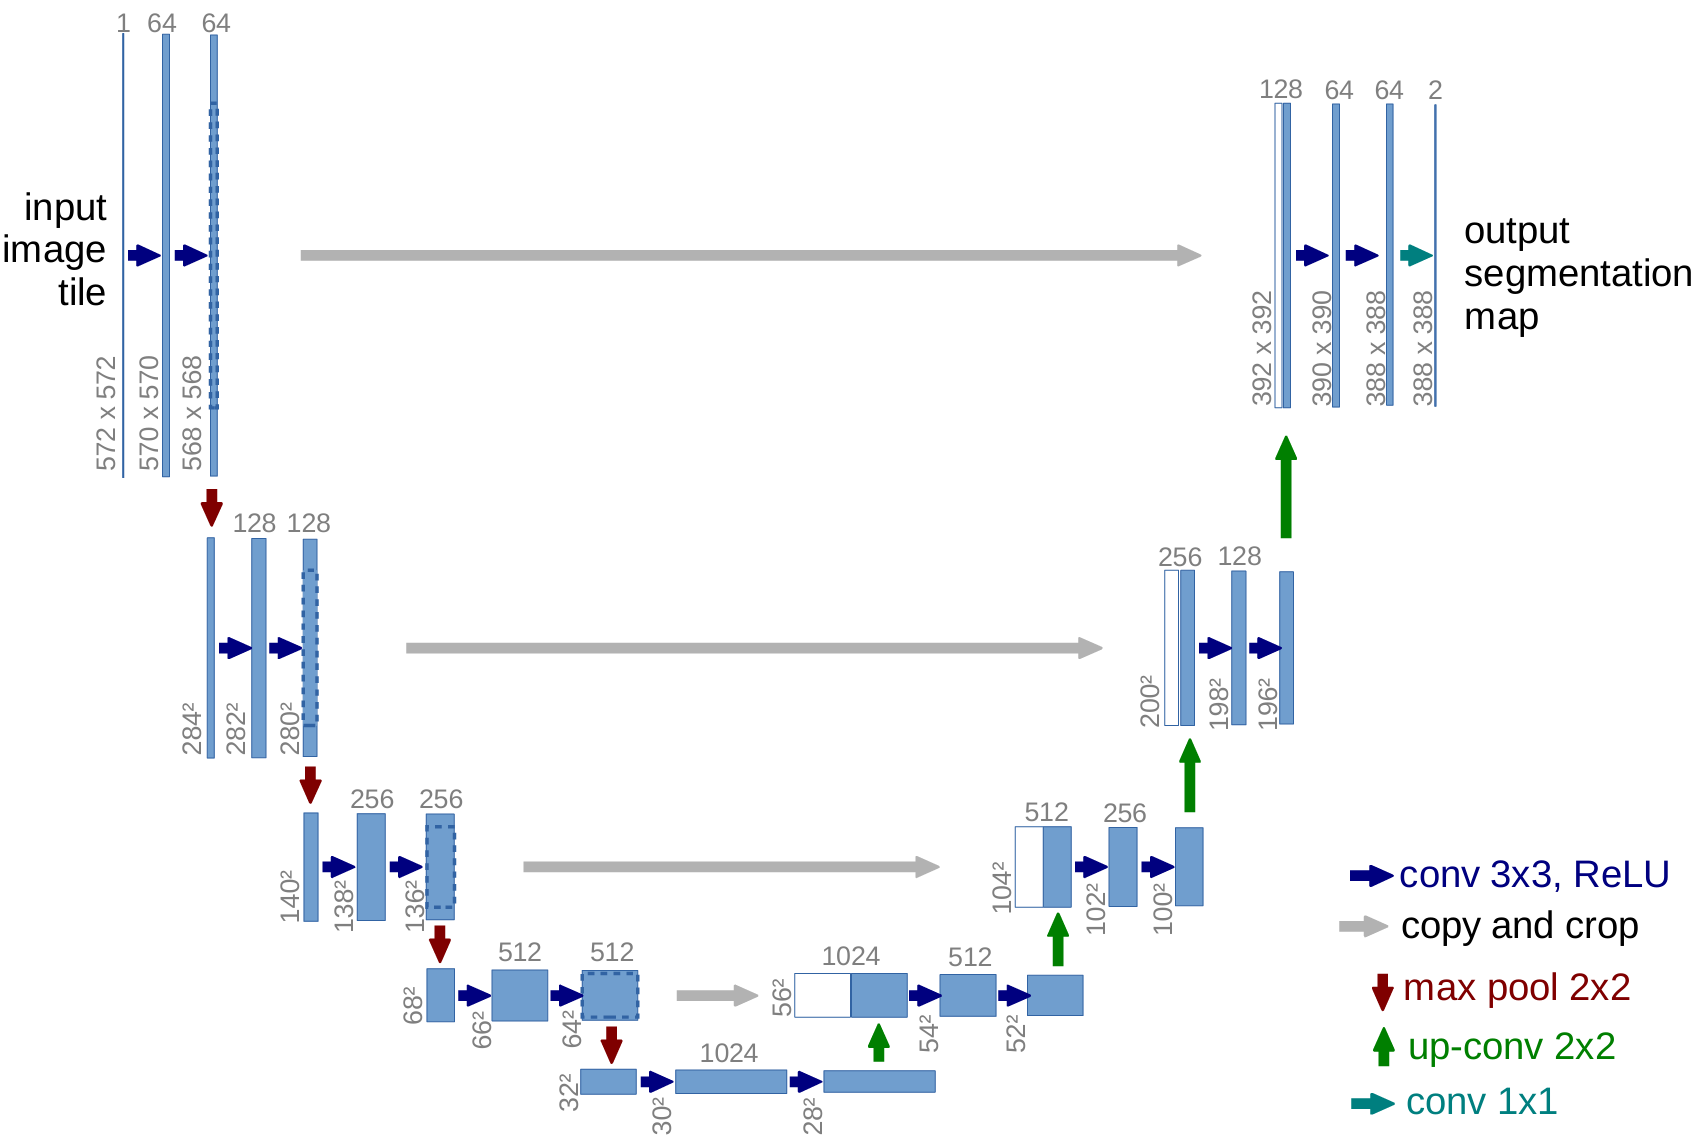
\includegraphics[width=12cm, height=8cm]{unet-architect.png}
	\caption{U-Net网络结构示意图}
	\label{unet-architect}
\end{figure}

其中,蓝色箭头表示一个卷积核尺寸为$3\times3$、无零填充、步长为1的卷积层,加上一个RuLU激活函数层的标准卷积操作。
红色箭头表示基于最大池化方法的下采样操作,主要用于实现特征图降维。
绿色箭头表示一个上采样升维和$2\times2$卷积的组合操作,其中上采样方法包括插值法和反卷积法,原作者采用的是双线性插值方法实现上采样,不涉及参数,只涉及计算。
灰色箭头表示先把编码器对应的输出特征图,按照通道维度拼接到当前特征图中,由于作者未做零填充,导致特征图宽高有所下降,故需要裁剪后再拼接。
最后输出层将64通道的特征图,通过$1\times1$卷积变换为双通道特征图,用于实现二分类的概率通道。本文即作为裂缝和背景两个类别的输出通道。

\subsection{U-Net关键特性}

\textbf{(1)Concat层}

Concat层一种跳连接算法,是U-Net卷积网中最重要的操作之一。它将编码器的对应输出特征图,按照特征通道的方向,拼接到解码器的对应特征图上,从而增加了解码器的特征图通道数量。

该层的关键作用是将编码器部分提取的浅层特征的位置信息和深层特征的语义信息进行了融合。
它在解码器恢复原始图像分辨率尺寸的过程中,获取更精确的位置信息,从而取得精确的像素位置还原。

这种特征图拼接的方式,相比分类网中特征图相加的方式,更好地保留了浅层的位置信息,这对于语义分割任务更为有效。


\textbf{(2)Encoder-Decoder结构}

U-Net卷积网的编码器-解码器结构,是当前深度学习模型经典、常见的结构类型。
其核心思想是将原始图像、文本等数据,通过编码器得到深层、高维的抽象表示,以提取数据最重要的特征信息;
再通过解码器对数据特征空间进行降维的过程,融合编码器输出的浅层特征,包括空间位置特征、时间序列特征等时空信息,还原图像的空间位置关系、文本的上下文依赖关系。

基于U-Net进行裂缝图像检测时,编码器Encoder会不断提取图像特征,输出背景、裂缝的高维、抽象的特征空间表达。
紧接着,解码器Decoder会在还原增大特征图尺寸和输出语义信息的同时,通过Concat拼接操作,融合编码器阶段输出的浅层特征的位置信息,从而准确还原背景、裂缝的语义和位置信息,获得位置精确的语义分割效果。


%————————————————————————————————————————————算法精度实验—————————————————————————————————————————————————————————————————————————
\section{算法性能实验及结果分析}
本节在PC端搭建实验环境和实验数据集,对U-Net卷积分割网进行模型参数训练、精度测试和实验结果对比分析,
以确保算法保持一定精度,为后续边缘部署和推理系统的设计、实现和系统推理时延实验奠定前提和基础。

\subsection{实验数据集}
\textbf{(1)数据集来源}

本文算法精度实验采用的数据集,采用自Yong Shi等人提出\citing{forest_detect}的随机结构森林实现裂缝检测的论文。

该数据集总共包含118张采集真实路面的裂缝图像,包括对应图像的标签。
其中,标签是对原图像的灰度化处理,它将背景处理为灰度值为0的黑色像素点,将裂缝处理为灰度值为255的白色像素点,
从而得到与118张数据集对应的掩码图。

在模型参数训练阶段,需要将标签掩码图转化为0-1的张量,并进行独热编码,用于损失函数计算。
该数据集原始图像与掩码图像,如下图所示:

\begin{figure}[H]
\subfloat[]{
    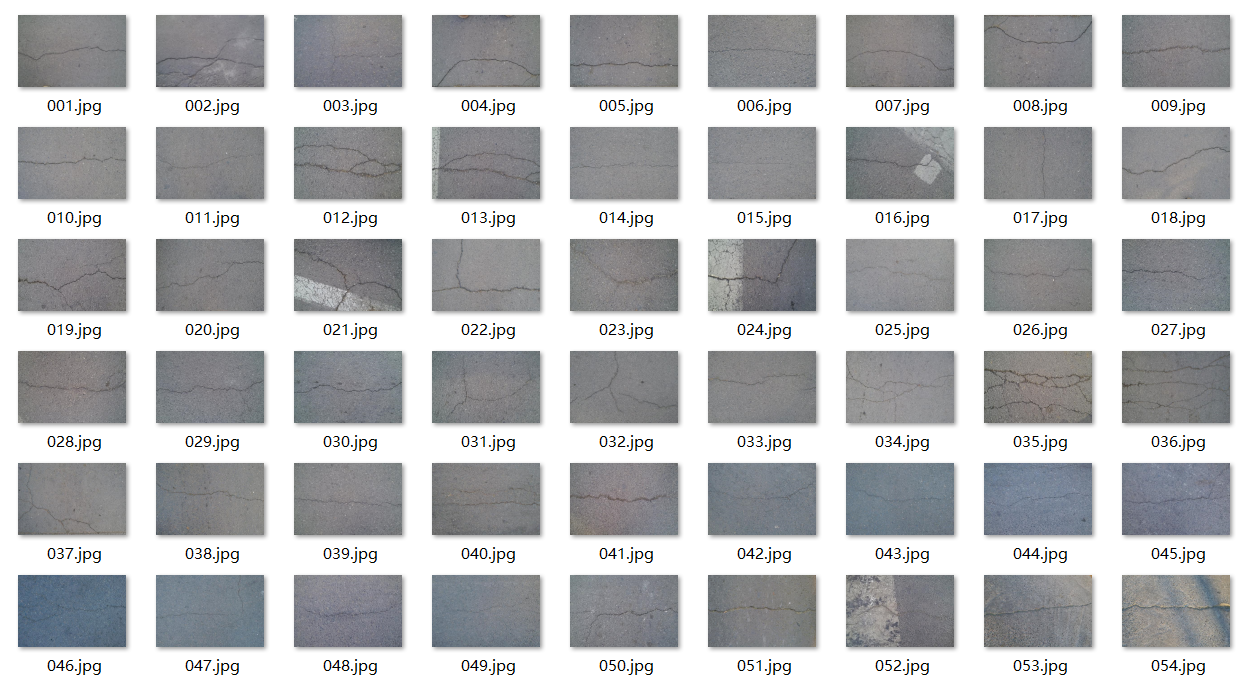
\includegraphics[width=7.5cm, height=5.5cm]{pic/dataset-crack.png} 
    \label{crack_png}
}
\subfloat[]{
    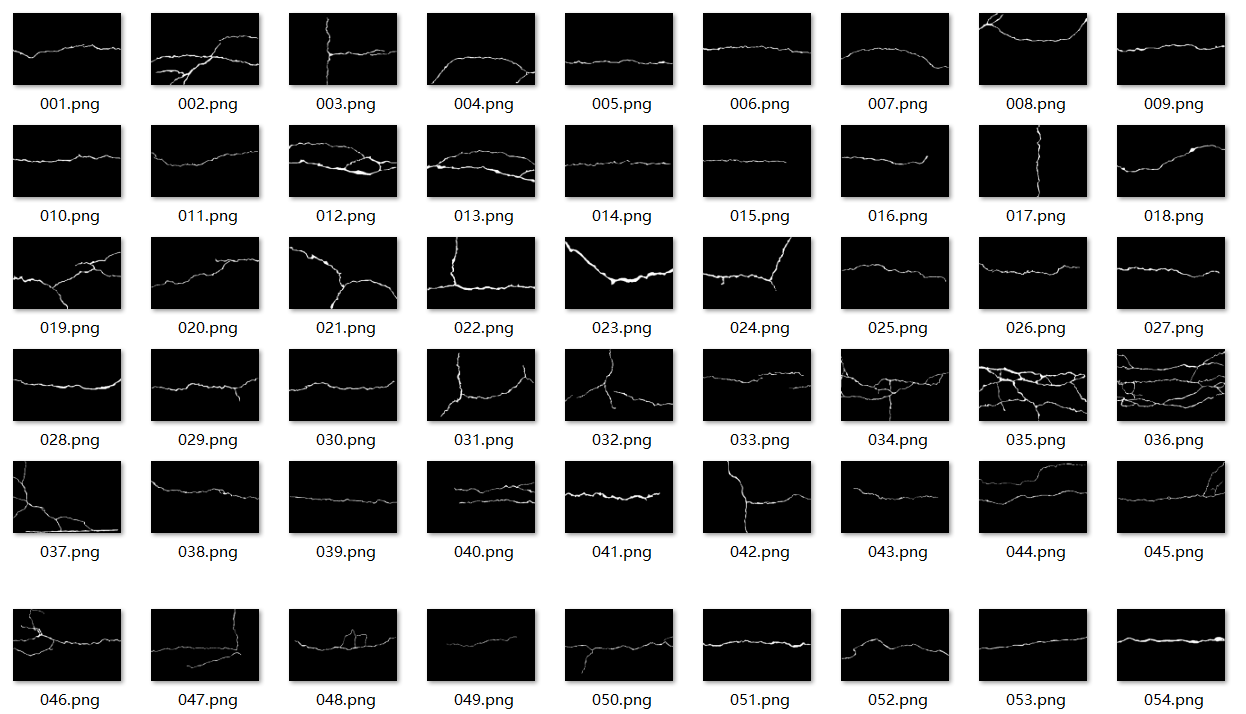
\includegraphics[width=7.5cm, height=5.5cm]{pic/dataset-musk.png}
    \label{musk_png}
}
\caption{图像和掩码数据集示意图}
\end{figure}

\textbf{(2)数据增广}

由于原始数据集只包含118张裂缝图像,本文采用数据增广技术,对原始数据集进行增强和数量扩充,以满足模型参数训练需求。
主要采取的数据增广方法包括上下翻转、左右翻转、上下+左右翻转、亮度增加、亮度减少、对比度增高和对比度降低。

经过图像增广操作,数据集从原始的118张扩大到了944张,数量增长了8倍,
数据的多样性也得到大幅增加。因此,经过增广后的数据集,更有利于模型参数拟合、加速模型收敛、提高模型鲁棒性和泛化能力。

上下翻转、亮度增加、对比度增加的效果图,如下图\ref{vertical}、\ref{brightness}、\ref{contrast}所示:

\begin{figure}[H]
\subfloat[]{
    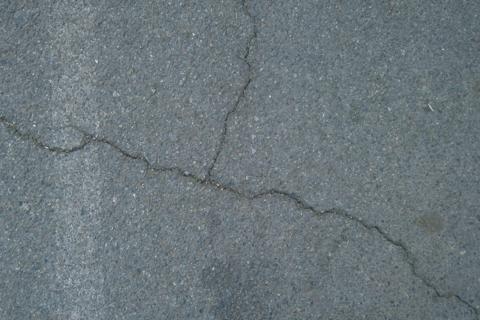
\includegraphics[width=6cm, height=4cm]{pic/origin_vertical.png}
    \label{origin_vertical}
}
\subfloat[]{
    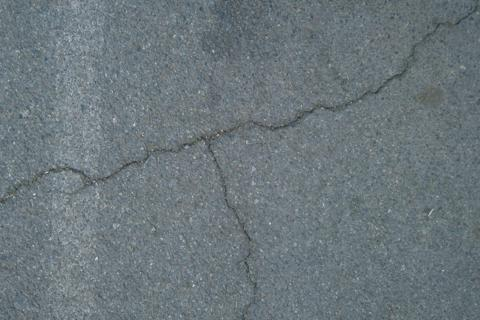
\includegraphics[width=6cm, height=4cm]{pic/agu_vertical.png} 
    \label{agu_vertical}
}
\caption{上下翻转效果图}
\label{vertical}
\end{figure}

\begin{figure}[H]
\subfloat[]{
    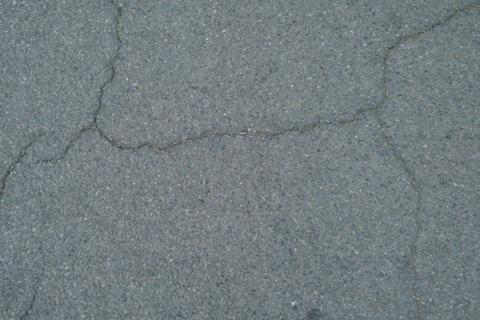
\includegraphics[width=6cm, height=4cm]{pic/origin_bright.png}       
    \label{origin_bright}
}
\subfloat[]{
    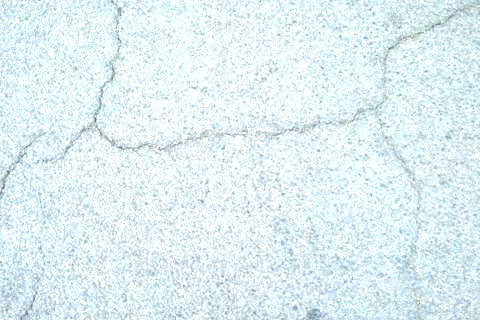
\includegraphics[width=6cm, height=4cm]{pic/agu_bright.png}
    \label{agu_bright}
}
\caption{亮度增加效果图}
\label{brightness}
\end{figure}

\begin{figure}[H]
\subfloat[]{
    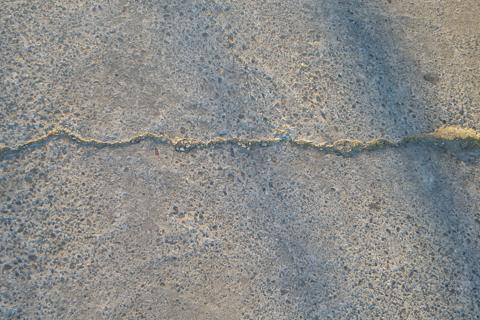
\includegraphics[width=6cm, height=4cm]{pic/origin_contrast.png}
    \label{origin_contrast}
}
\subfloat[]{
    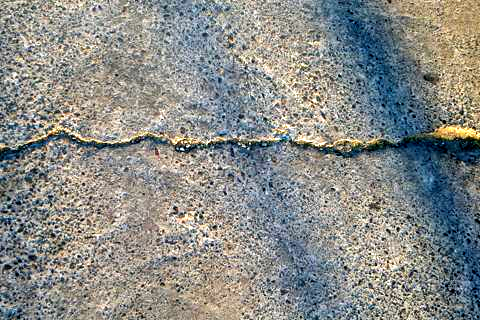
\includegraphics[width=6cm, height=4cm]{pic/agu_contrast.png}    
    \label{agu_contrast}
    }
\caption{对比度增加效果图}
\label{contrast}
\end{figure}


\subsection{实验设置}
本文的道路裂缝数据集基于80\%、10\%、10\%的占比,划分为裂缝检测训练集、验证集以及测试集。
其中,训练集用于模型参数训练。
验证集用于模型验证并根据验证指标适时保存模型参数和训练叫停,避免模型过拟合。
测试集用于模型精度等指标的测试和实验。

模型训练采用交叉熵损失函数衡量损失,使用Adam优化器进行学习率动态调整、参数更新和寻找最优值。
训练时,每批次batch大小设置为8,初始学习率为0.00001,训练轮数epochs取200轮。

模型算法采用Python3.8编写,深度学习框架为GPU版本PyTorch2.0.0,操作系统为Ubuntu20.04,CUDA版本为11.8,
CPU为Intel(R) Xeon(R) CPU E5-2680 v4 @2.40GHz,
采用的显卡为NVIDIA GeForce RTX3090,
内存大小为256GB,显存大小为24GB。

本节所有算法精度实验,均基于上述数据集、训练参数和实验平台开展。

\subsection{评价指标}
本章提出的算法是图像分割网,基于该类型的特点,采用准确率precision、召回率recall、F1得分f1-score作为算法精度的评价指标,
下面对这三项评价指标做出详细介绍:

\textbf{(1)混淆矩阵}

在深度学习分类任务中,对一个事物分类的结果可以使用混淆矩阵(Confusion Matrix)进行表示,帮助我们只管地理解模型的分类表现。

在二分类问题中,预测和实际类别分为正类Positive、负类Negative两类,对某个事物的二分类结果可以使用
如下的矩阵结构进行表示:

\begin{figure}[H]
	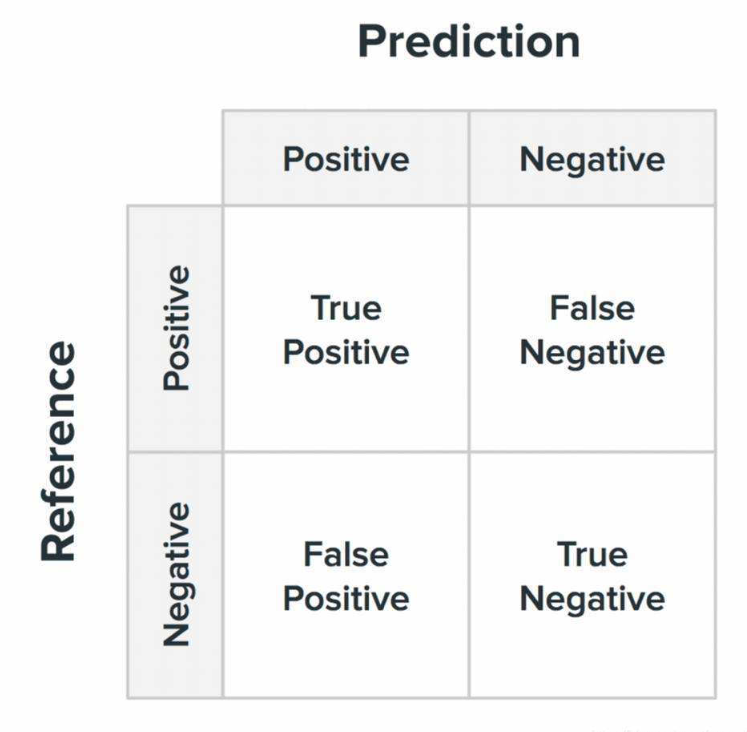
\includegraphics[width=10cm, height=8cm]{pic/confusion-matrix.png}
	\caption{混淆矩阵结构示意图}
	\label{confusion-matrix}
\end{figure}

其中,实际和预测的类别被分成正类别Positive、负类别Negative。
TP,True Positive表示正类被正确预测为正类;
FP,False Positive表示负类被错误预测为正类;
FN,False Negative表示正类被错误预测为负类;
TN, True Negative表示负类被正确预测为负类。

在多分类任务中,若类别为$n$类,则混淆矩阵是$n\times n$维矩阵,其中元素$(i,j)$表示类别$i$被预测为类别$j$的个数。

在本文中,图像每个像素会被预测为裂缝和背景两个类别。

\textbf{(2)准确率precision}

准确率(precision)指的是某一类别的样本中预测正确的样本数的占比。
在本文实验中,准确率是模型在实际为裂缝类的像素样本中,预测正确的样本数占比。
准确率的计算公式如下,其中TP、TN、FN为对应预测结果的样本数量,下同。

\begin{equation}
    precision=\frac{TP}{TP+FP}
\end{equation}

\textbf{(3)召回率recall}

召回率(recall)指的是预测为某一类别的样本中预测正确的样本数占比。
在本文实验中,召回率是模型预测为裂缝的像素样本中,实际是裂缝类的样本数占比。
召回率的计算公式如下:

\begin{equation}
    recall=\frac{TP}{TP+FN}
\end{equation}

\textbf{(4)F1得分f1-score}

F1得分(f1-score)是准确率和召回率两个指标的调和平均数,综合考虑了这两个指标。
因为在实际分类任务中,可能出现准确率很高,但召回率很低的情况,比如将其他类也预测成了裂缝类;
也可能出现准确率很低,但召回率很高的情况,比如只将极少量的裂缝类样本预测出来。

F1得分的计算公式如下:
\begin{equation}
    f~1{-}score=2\times\frac{precision\times{recall}}{precision+recall}
\end{equation}

\subsection{算法精度测试}

\textbf{(1)测试结果与得分}

基于参数训练完成的模型,选取2张测试集裂缝图片,对模型检测精度进行测试,
测试效果如下图\ref{test-1}、\ref{test-2}所示:

\begin{figure}[H]
    \subfloat[]{
        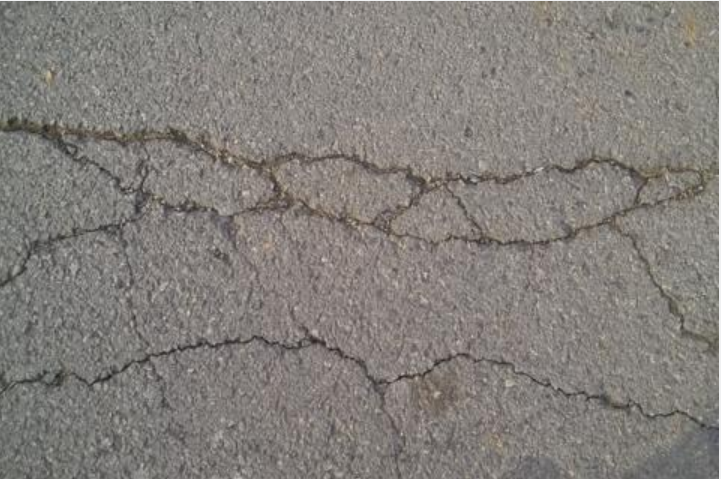
\includegraphics[width=6cm, height=4cm]{pic/crack-1-origin.png}
        \label{crack-1-origin}
    }
    \subfloat[]{
        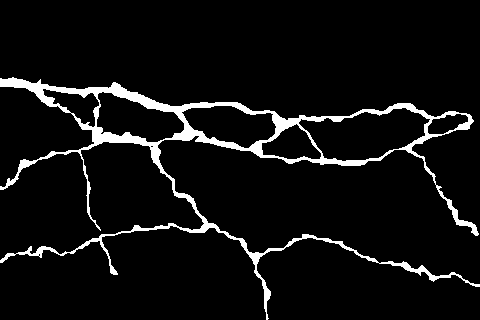
\includegraphics[width=6cm, height=4cm]{pic/crack-1-result.png} 
        \label{crack-1-result}
    }
    \caption{测试集裂缝图片\ding{172}测试结果图}
    \label{test-1}
\end{figure}

\begin{figure}[H]
    \subfloat[]{
        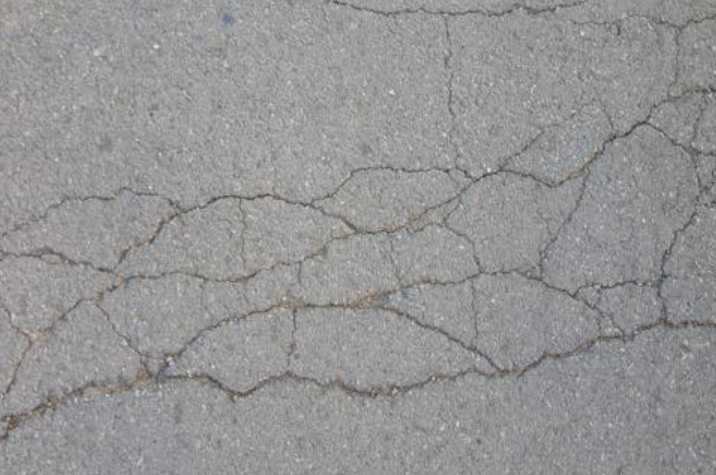
\includegraphics[width=6cm, height=4cm]{pic/crack-2-origin.png}
        \label{crack-2-origin}
    }
    \subfloat[]{
        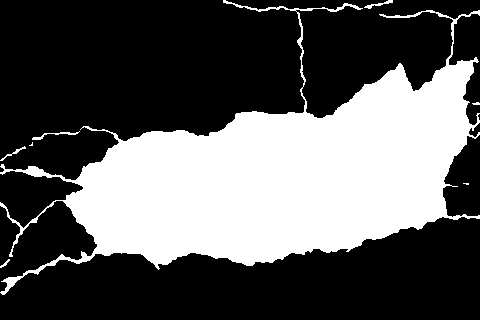
\includegraphics[width=6cm, height=4cm]{pic/crack-2-result.png}
        \label{crack-2-result}
    }
    \caption{测试集裂缝图片\ding{173}测试结果图}
    \label{test-2}
\end{figure}

上述两张图分别展示了模型对裂缝图片\ding{172}和裂缝图片\ding{173}的测试效果,
可以看到,裂缝的细节处理得当,识别效果较好,算法检测精度较好。

下表将增加两张测试图片,给出4张测试集图片的各指标相应的测试得分,见下表\ref{test-score}所示:

\begin{table}[H]
    \scriptsize
    \caption{测试集各指标得分}
    \label{test-score}
    \begin{tabular}{>{\centering\arraybackslash}p{3cm}>{\centering\arraybackslash}p{3cm}>{\centering\arraybackslash}p{3cm}>{\centering\arraybackslash}p{3cm}}
    \toprule
     图片序号  & Precision & Recall & F1-Score \\ 
    \midrule
    \ding{172} & 0.9234    & 0.9325 & 0.9413   \\
    \ding{173} & 0.9156    & 0.9311 & 0.9326   \\ 
    \ding{174} & 0.9213    & 0.9276 & 0.9288   \\ 
    \ding{175} & 0.9357    & 0.9389 & 0.9341   \\ 
    \bottomrule
    \end{tabular}
\end{table}

根据测试结果图和测试得分可知,模型的泛化能力和检测精度较高。

本文U-Net模型精度提升的主要贡献,来自对原始数据集进行的数据增广,包括仿射变换和色彩变换两类数据增广技术。
下文将随机选取测试集中的的一张裂缝图片,给出数据增广前后的测试结果图和相应得分的对比。

\textbf{(2)原始数据集测试结果}

原始数据集,测试结果如下图:
\begin{figure}[H]
    \subfloat[]{
        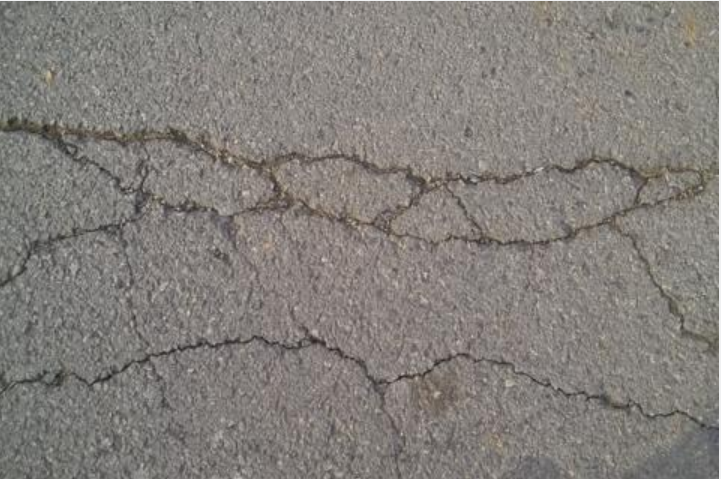
\includegraphics[width=6cm, height=4cm]{pic/crack-1-origin.png}
        \label{crack-a-1}
    }
    \subfloat[]{
        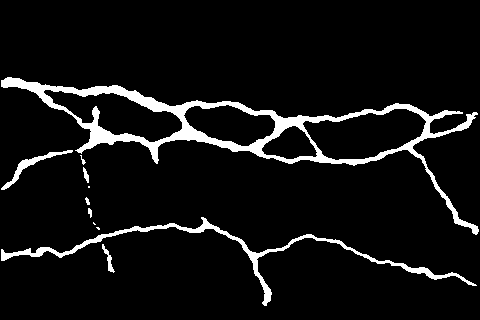
\includegraphics[width=6cm, height=4cm]{pic/crack-origin.png} 
        \label{crack-a-2}
    }
    \caption{原始数据集测试结果图}
    \label{test-origin}
\end{figure}

\textbf{(3)仿射变换后测试结果}

原始数据集+仿射变换,测试结果如下图:
\begin{figure}[H]
    \subfloat[]{
        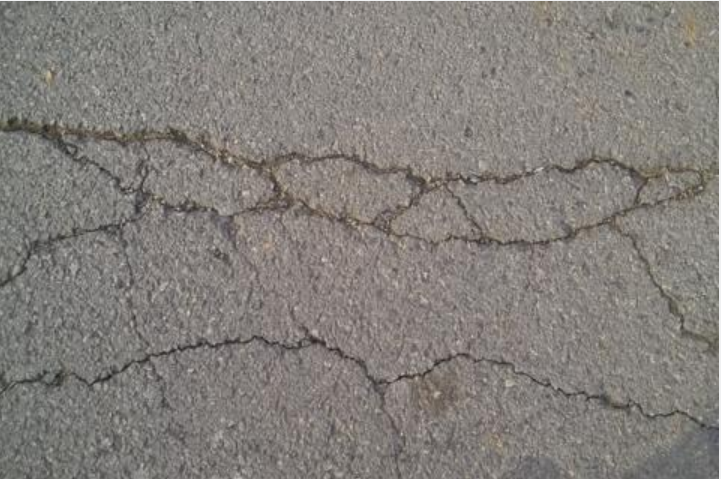
\includegraphics[width=6cm, height=4cm]{pic/crack-1-origin.png}
        \label{crack-b-1}
    }
    \subfloat[]{
        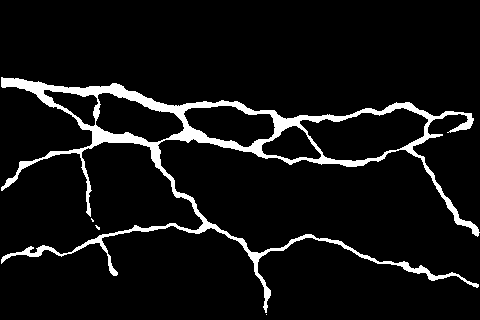
\includegraphics[width=6cm, height=4cm]{pic/crack-geometry.png}
        \label{crack-b-2}
    }
    \caption{原始数据集+仿射变换测试结果图}
    \label{test-geometry}
\end{figure}

经过上下翻转、水平翻转、上下水平翻转的仿射变换操作后,数据集从118张增加到了472张,增长为原来的4倍。
根据上图可知,仿射变换后的数据集训练得到的模型,对裂缝识别效果更好,裂缝细节识别更加清晰。

\textbf{(4)色彩变换后测试结果}

原始数据集+仿射变换+色彩变换,测试结果如下图:
\begin{figure}[H]
    \subfloat[]{
        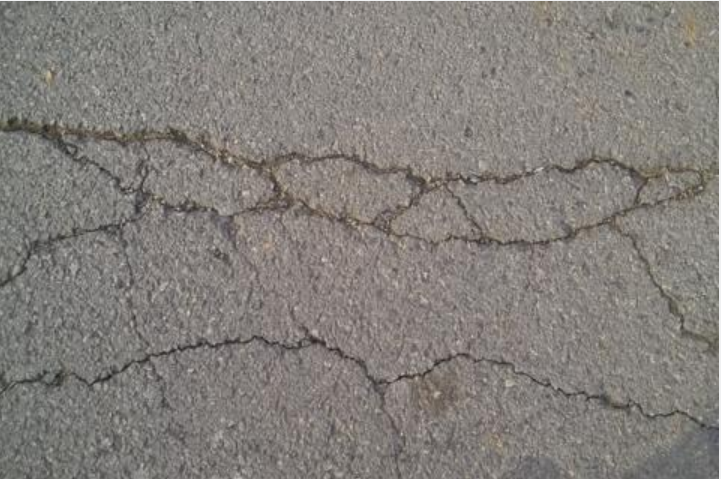
\includegraphics[width=6cm, height=4cm]{pic/crack-1-origin.png}
        \label{crack-c-1}
    }
    \subfloat[]{
        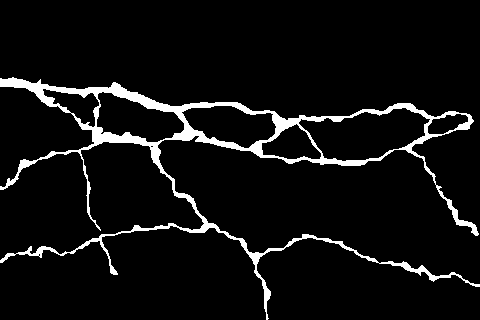
\includegraphics[width=6cm, height=4cm]{pic/crack-geometry-color.png}
        \label{crack-c-2}
    }
    \caption{原始数据集+仿射变换+色彩变换测试结果图}
    \label{test-geometry-color}
\end{figure}

在仿射变换基础上,再经过亮度增加、亮度降低、对比度增加、对比度降低的色彩变换操作后,数据集从118张增加到了944张,增长为原来的8倍。
根据上图可知,色彩变换后的数据集训练得到的模型,对裂缝识别效果进一步提升,裂缝细节的识别也进一步清晰。

\textbf{(5)数据增广前后得分对比}

接下来给出数据增广前后,该测试集图片裂缝识别各指标的得分结果,如下表所示:

\begin{table}[H]
    \scriptsize
    \caption{数据增广前后各指标得分}
    \label{test-score-agument}
    \begin{tabular}{>{\centering\arraybackslash}p{6cm}>{\centering\arraybackslash}p{2cm}>{\centering\arraybackslash}p{2cm}>{\centering\arraybackslash}p{2cm}}
    \toprule
    数据集类型   & Precision & Recall & F1-Score \\ 
    \midrule
    原始数据集    & 0.7576    & 0.7469 & 0.7522   \\
    原始数据集+仿射变换    & 0.7960    & 0.7941 & 0.7938   \\ 
    原始数据集+仿射变换+色彩变换  & 0.9234    & 0.9325 & 0.9413   \\ 
    \bottomrule
    \end{tabular}
\end{table}

根据上表测试指标得分可知,经过对原始数据集进行仿射变换后,模型在测试集图片上识别得分提高了接近4个百分点;
在仿射变换基础上,对原始数据集再进行色彩变换后,模型在测试集图片上识别得分提高了近14个百分点,模型识别能力显著提升。

\textbf{(6)结果分析}

根据上述实验结果可知,数据集的数量和多样性,对于模型泛化能力、精度、鲁棒性的提升十分重要。
大量且多样的数据集,有利于模型进一步学习裂缝特征的不变性,增强其对裂缝的分类和检测能力。


%————————————————————————————————————————————本章小结—————————————————————————————————————————————————————————————————————————
\section{本章小结}
本章介绍了基于U-Net的边缘智能裂缝检测算法设计与实现。
首先,介绍了边缘智能裂缝检测系统所采用的深度学习算法——基于U-Net的卷积神经网络分割网,并详细阐释了U-Net的两个关键特性,分别是跳连接层Concat和编解码Encoder-Decoder结构。
紧接着,对原始数据集应用了仿射变换、色彩变换等数据增广技术。增广后的数据集,不仅数量得到增加,而且数据多样性也得以增加,这对模型泛化能力和鲁棒性的提升十分重要。
最后,基于增广后的数据集对模型进行了参数训练,并使用测试集对模型精度得分、增广前后精度得分等进行了实验、对比和结果分析。